\section{Technical Design}\label{sec:technical-design}
%\lipsum[2-8]
At the end of section:~\ref{sec:op-params} it was shown that using the raw position readings coming from the sensor is not feasbile in cases where NLOS is present.
Furthermore, the overall goal is for the position of an indoor UAV to be recovered with a fair amount of accuracy since this forms the basis of any autonomous behaviour and navigation.
As such it is desirable to use readings from multiple sensors but at the same time of reducing the overall physical footprint of the final system to keep it lightweight.
With that in mind it is proposed to directly integrate the POZYX sensor system with a motherboard unit that is capable of doing sensor fusion, UAV control and communicating with external systems.
In recent years FCU's have become versatile and robust and these requirements are easily met so in this section the technical parameters of the research will be discussed.

\subsection{Flight Controller Unit}\label{subsec:flight-controller-unit}
In order to prevent consuming too much time on dertermining a suitable flight system the Open-Source Hardware (OSH) community was consulted in order to find a suitable FCU for the research.
Survey work done by ~\citet{ebeid2018survey} present a qualitative analysis of several commercial hardware solutions.
Table:~\ref{tb:comparison} shows some of the major hardware considerations.
All of the units have the standard UART, PWM and I2C interfaces in addition to other onboard sensors and interfaces.
At the time of writing the Pixhawk series of FCU's are the most common and oldest systems.
They have all the standard interfaces as well as several sensors allowing making them a keen choice for developers and researchers in a plug and play platform.
Many in the series share the same intefaces with some of the smaller boards excluding some of the less popular interfaces.
As such, to allow for flexibility in the technical design one of the Pixhawk family was desirable for this research.
After deliberation and consulting the objectives and scope of this research it was determined that a basic Pixhawk would be satiable.
Figure:~\ref{fig:pix} shows the board chosen, it was shipped quickly and it contains everything necessary to meet the objectives of the project allowing for quick prototyping and proof of concepts.

\begin{table}[h!]
    \centering
    \begin{tabular}{|c | c | c | c | c|}
        \hline
        Platform & MCU & Sensors & Licenses & Interfaces\\
        \hline
        Pixhawk & STM32F427 & b, m & BSD & c, s, a, pp, sb, ds\\

        Pixhawk2 & STM32F427 & b, m & CC-BYSA-3.0 & c, s, a, pp, sb, ds\\

        PixRacer & STM32F427 & b' m & CC-BY 4.0 & c, pp, sb, ds \\

        Pixhawk 3 Pro & STM32F427 & b' m & CC-BY 4.0 & c, s, pp, sb, ds \\

        PX4 FMUv5 and v6 & STM32F427 & b' m & CC-BY 4.0 & c, s, a, pp, sb, ds \\

        CC3D & STM32F103 & None & GPLv3 & pp, ds, sb\\

        APM 2.8 & ATmega2560 & b & GPLv3 & pp, a\\

        Erle-Brain 3 & Raspberry Pi & b, m & CC BY-NC-SA &  a\\

        PXFmini & Raspberry Pi & b, m & CC BY-NC-SA & a\\
        \hline
    \end{tabular}
    \caption{Comparisons of various FCU's that are commercially available. Source: ~\citet{ebeid2018survey} Page: 2.}
    \label{tb:comparison}
    b: barometer, m: magnetometer, p: pitot tube sensor, c: CAN, s: SPI, a: ADC, pp:
PPM, sb: S.BUS, ds: DSM, da: DAC, x: XBEE, au: AUX, [d]: discontinued.
\end{table}

\begin{figure}[ht!]
    \centering
    \includegraphics[scale=0.7]{mtd/pixhawk}
    \caption{Radiolink Pixhawk used for the project}
    \label{fig:pix}
\end{figure}

Furthermore, since the chosen board is OSH it has several options of firmware that can be used which makes code and software developed on this system extendable to other boards given they are able to run the firmware.
\newpage

\subsection{Flight Firmware}\label{subsec:flight-firmware}
Now that a suitable FCU was chosen the next major step was determining a flight stack to run on the board.
The major firmware options for the Pixhawk are either Ardupilot or PX4 stack.
Both are well documented and have their advantages.
Both support a large array of vehicles but the major differences come from the licenses they are under.
Without delving into the technicalities of the licenses it is often summarised that PX4 is attractive to business owners who want to protect their property whilst Ardupilot pushes for changes to be put back into the main codebase.
Additionally, from a quick brief and use of each of the firmwares, Ardupilot is slightly more documented due to its general public license and a bit more user friendly in terms of compilation and flashing firmware thanks to its pythonic based wrapper for compilation and uploading.
Since both firmwares cover all the generic UAV types and there was no need for any niche systems Ardupilot was chosen as the primary codebase.
It is worth noting that there is a subsection of the Ardupilot codebase is dedicated to Beacon based positioning systems which a previous Pozyx implementation is coded ~\cite{ardupilotarduino}.

\subsection{Communication Interface (I2C vs Serial)}\label{subsec:communication-interfacei2c-vs-serial}
As mentioned in Chapter:~\ref{ch:literature-review} there is an implementation of using a Pozyx system in a GPS denied scenario ~\cite{ardupilotarduino}.
This shows that it is possible to get the positioning data into the Ardupilot codebase and have it interacting with the onboard sensor fusion systems.
A critique of this approach however is that it uses an additional Arduino Uno to pipe information from the Pozyx tag to the Pixhawk.
Given the availability of the standard interfaces onboard the Pixhawk and the scope and objectives of this research project it is feasible that the Uno can be stubbed out of this experiment and data can be integrated directly onto the Pixhawk.
This means the physical integration of the system can be summarised into the following steps:
\begin{itemize}
    \item Choose a suitable interface.
    \item Place the code within a suitable section of the codebase.
    \item Utilise the parent class of the section of the Ardupilot to integrate the sensor.
    \item After testing the base functionality, integrate the new library within the background scheduler so it can run and feed measurements in the background to the copter main code.
\end{itemize}

An Arduino ~\cite{pozarduino} and python library was originally designed by the Pozyx developers so it provided an algorithmic starting point for the functionality of the library being designed.
The Arduino library is based around the I2C protocol whilst the python module uses the serial interface.
As noted by the developers the python module is a port of the Arduino library and there is no plans to maintain the code and address bug fixes, as such the Arduino library was studied fo to build the new AP\_Bacon extension.
Furthermore, the I2C interface was designed onboard an embedded system so much of the flow can be ported effectively to the Pixhawk.
Lastly, the previous implementation uses the UART/serial interface so that avenue has already been explored so in the intrest of quick prototyping the I2C interface was chosen.
A positive note is that the existence of the prebuilt system allows data and experiments to be collected in lieu of development of this library since the information being provided is the same data generated by the Pozyx tag.
The design of this library proves that the sensor data can be integrated directly whilst the pre-built systems, which are stable, can be used for data collection and experiments.
%
%\begin{figure}[h!]
%    \centering
%    \includegraphics[scale=0.5]{}

%\end{figure}

\begin{figure}[ht!]
    \centering
    \includegraphics[width=\textwidth]{mtd/pozyx_uno}
    \caption{Non-GPS loiter solution provided by Ardupilot. Soruce:\url{https://ardupilot.org/copter/docs/common-pozyx.html}}
    %    \label{fig:pix}
\end{figure}

\begin{figure}[ht!]
    \centering
    \includegraphics[scale=0.6]{mtd/i2c_ifc}
    \caption{Proposed wiring of the I2C interface being developed}
\end{figure}

\begin{figure}[ht!]
    \centering
    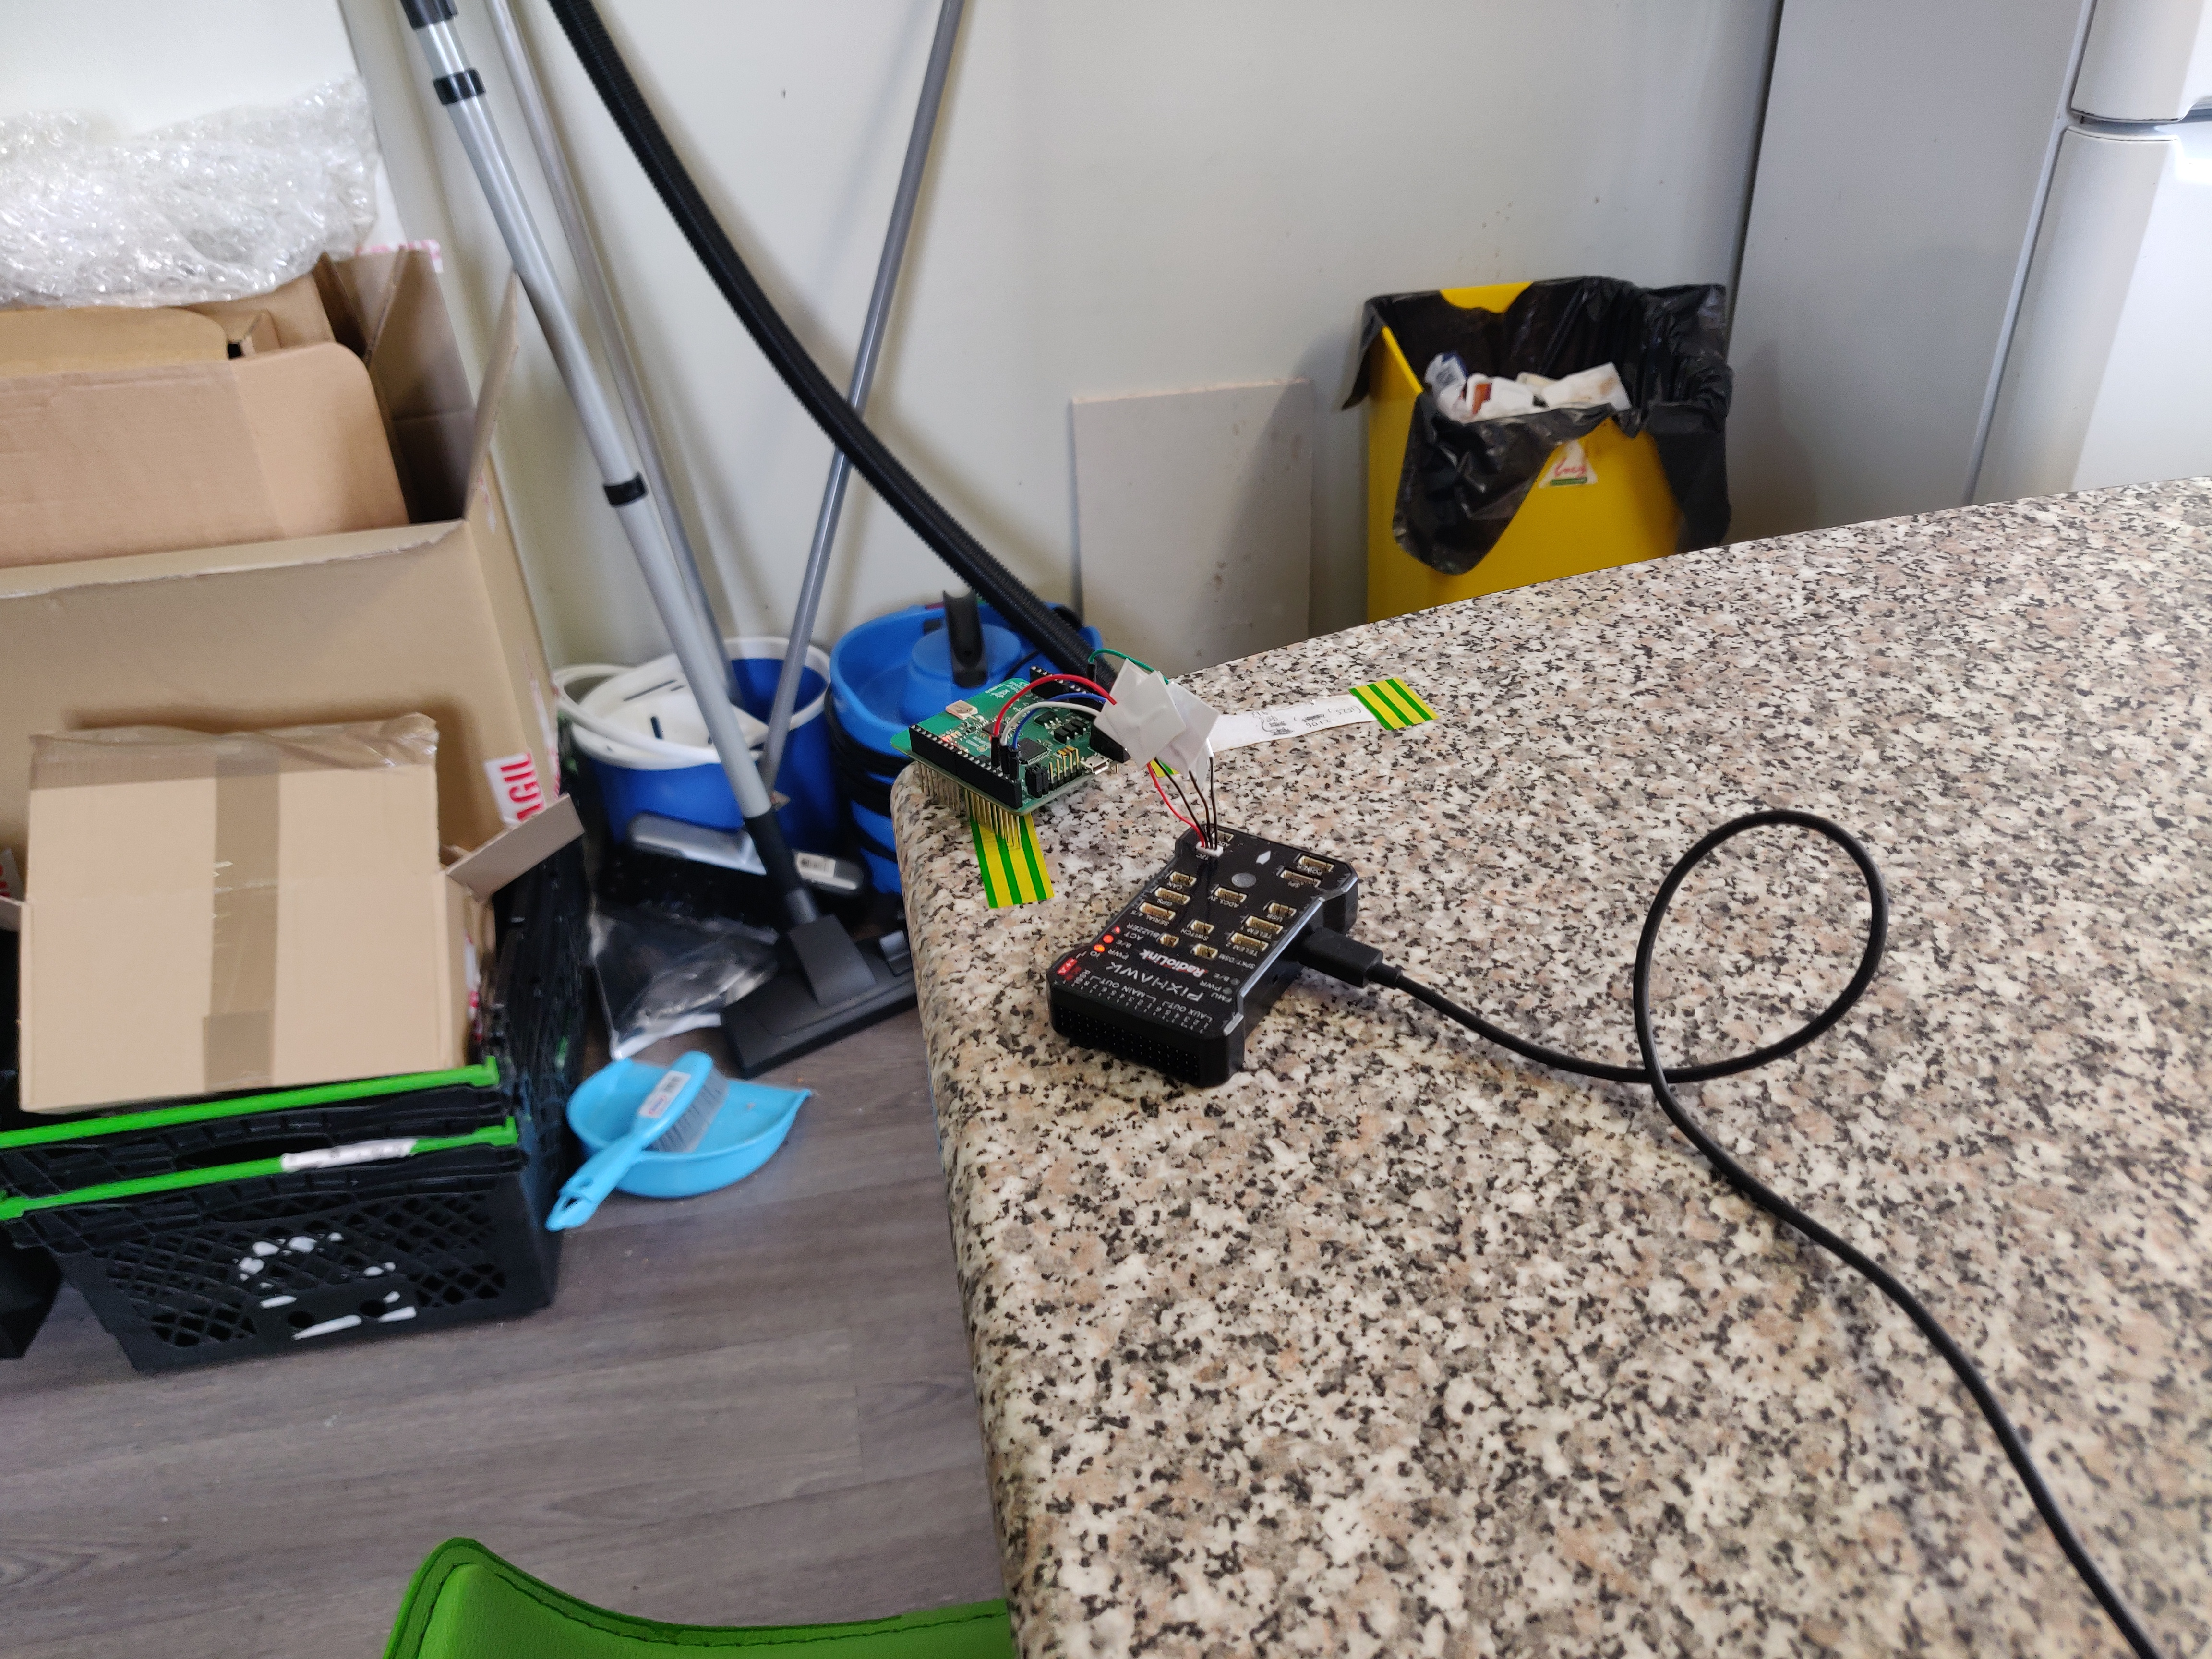
\includegraphics[width=\textwidth]{mtd/wip}
    \caption{System being unit tested in the environment.}
\end{figure}
\newpage
\subsection{Sensor Fusion: EKF on Ardupilot}\label{subsec:sensor-fusion}
\lipsum[2-6]